\addchap[Appendix C:$\quad$3D Graphing with Gnuplot]{Appendix C}
\textsf{\textbf{\Large 3D Graphing with Gnuplot}}\vspace{4mm}

Gnuplot is a free, open-source software package for producing a variety of graphs. Versions are available for many
operating systems. Below is a very brief tutorial on how to use Gnuplot to graph functions of several
variables.\vspace{4mm}

\par\noindent\textbf{INSTALLATION}
\begin{enumerate}
 \item Go to \url{http://www.gnuplot.info/download.html} and follow the links to download the latest version for your
  operating system. For Windows, you should get the Zip file with a name such as \path{gp420win32.zip}, which is
  version 4.2.0. 
  All the examples we will discuss require at least version 4.2.0.
 \item Install the downloaded file. 
 For example, in Windows you would unzip the Zip file you downloaded
  in Step 1 into some folder (use the ``Use folder names'' option if extracting with WinZip).
\end{enumerate}

\par\noindent\textbf{RUNNING GNUPLOT}
\begin{enumerate}
 \item In Windows, run \textbf{\path{wgnuplot.exe}} from the folder (or \path{bin} folder)
  where you installed Gnuplot. In Linux, just type
  \textbf{\path{gnuplot}} in a terminal window.
 \item You should now get a Gnuplot terminal with a \textbf{\path{gnuplot>}} command prompt. In Windows this
  will appear
  in a new window, while in Linux it will appear in the terminal window where the \textbf{\path{gnuplot}} command was
  run. For Windows, if the font is unreadable you can change it by right-clicking on the text part of the Gnuplot window
  and selecting the ``Choose Font..'' option. For example, the font ``Courier'', style ``Regular'', size ``12'' is
  usually a
  good choice (that choice can be saved for future sessions by right-clicking in the Gnuplot window again and selecting
  the option to update wgnuplot.ini).
 \item At the \textbf{\path{gnuplot>}} command prompt you can now run graphing commands, which we will now
  describe.
\end{enumerate}

\par\noindent\textbf{GRAPHING FUNCTIONS}\vspace{2mm}\\
The usual way to create 3D graphs in Gnuplot is with the \textbf{splot} command:
\begin{displaymath}
 \text{splot <range> <comma-separated list of functions>}
\end{displaymath}
For a function $z=f(x,y)$, <range> is the range of $x$ and $y$ values (and optionally the range of $z$ values) over
which to plot.
To specify an $x$ range and a $y$ range, use an expression of the form
\symbol{91}$a:b$\symbol{93}\symbol{91}$c:d$\symbol{93}, for some numbers $a<b$ and $c<d$. This will cause the graph to
be plotted for $a\le x\le b$ and $c\le y \le d$.\vspace{2mm}

\par\noindent Function definitions use the $x$ and $y$ variables in combination with mathematical operators,
listed below:\vspace{1mm}

\begin{center}
\begin{tabular}{@{} | c | c | c | c | @{}}
 \hline \textbf{Symbol} & \textbf{Operation} & \textbf{Example} & \textbf{Result}\\
 \hline $+$ & Addition & $2 + 3$ & $5$\\
 \hline $-$ & Subtraction & $3 - 2$ & $1$\\
 \hline * & Multiplication & $2$*$3$ & $6$\\
 \hline $/$ & Division & $4/2$ & $2$\\
 \hline ** & Power & $2$**$3$ & $2^3 = 8$\\
 \hline exp($x$) & $e^x$ & exp($2$) & $e^2$\\
 \hline log($x$) & $\ln x$ & log($2$) & $\ln 2$\\
 \hline sin($x$) & $\sin x$ & sin(pi/$2$) & $1$\\
 \hline cos($x$) & $\cos x$ & cos(pi) & $-1$\\
 \hline tan($x$) & $\tan x$ & tan(pi/$4$) & $1$\\\hline
\end{tabular}\end{center}

\vspace{2mm}
\hrule width \textwidth height 0.5pt\vspace{2mm}
\par\noindent \emph{\textbf{Example C.1.}}
 To graph the function $z = 2x^2 + y^2$ from $x=-1$ to $x=1$ and from $y=-2$ to $y=2$, type this at the
 \textbf{\path{gnuplot>}} prompt:
 \begin{displaymath}
  \texttt{splot \symbol{91}-1:1\symbol{93}\symbol{91}-2:2\symbol{93} 2*x**2 + y**2}
 \end{displaymath}
 The result is shown below:\vspace{-12mm}
\begin{figure}[h]
 \begin{center}
  % GNUPLOT: LaTeX picture with Postscript
\begingroup
\footnotesize
  \makeatletter
  \providecommand\color[2][]{%
    \GenericError{(gnuplot) \space\space\space\@spaces}{%
      Package color not loaded in conjunction with
      terminal option `colourtext'%
    }{See the gnuplot documentation for explanation.%
    }{Either use 'blacktext' in gnuplot or load the package
      color.sty in LaTeX.}%
    \renewcommand\color[2][]{}%
  }%
  \providecommand\includegraphics[2][]{%
    \GenericError{(gnuplot) \space\space\space\@spaces}{%
      Package graphicx or graphics not loaded%
    }{See the gnuplot documentation for explanation.%
    }{The gnuplot epslatex terminal needs graphicx.sty or graphics.sty.}%
    \renewcommand\includegraphics[2][]{}%
  }%
  \providecommand\rotatebox[2]{#2}%
  \@ifundefined{ifGPcolor}{%
    \newif\ifGPcolor
    \GPcolortrue
  }{}%
  \@ifundefined{ifGPblacktext}{%
    \newif\ifGPblacktext
    \GPblacktexttrue
  }{}%
  % define a \g@addto@macro without @ in the name:
  \let\gplgaddtomacro\g@addto@macro
  % define empty templates for all commands taking text:
  \gdef\gplbacktext{}%
  \gdef\gplfronttext{}%
  \makeatother
  \ifGPblacktext
    % no textcolor at all
    \def\colorrgb#1{}%
    \def\colorgray#1{}%
  \else
    % gray or color?
    \ifGPcolor
      \def\colorrgb#1{\color[rgb]{#1}}%
      \def\colorgray#1{\color[gray]{#1}}%
      \expandafter\def\csname LTw\endcsname{\color{white}}%
      \expandafter\def\csname LTb\endcsname{\color{black}}%
      \expandafter\def\csname LTa\endcsname{\color{black}}%
      \expandafter\def\csname LT0\endcsname{\color[rgb]{1,0,0}}%
      \expandafter\def\csname LT1\endcsname{\color[rgb]{0,1,0}}%
      \expandafter\def\csname LT2\endcsname{\color[rgb]{0,0,1}}%
      \expandafter\def\csname LT3\endcsname{\color[rgb]{1,0,1}}%
      \expandafter\def\csname LT4\endcsname{\color[rgb]{0,1,1}}%
      \expandafter\def\csname LT5\endcsname{\color[rgb]{1,1,0}}%
      \expandafter\def\csname LT6\endcsname{\color[rgb]{0,0,0}}%
      \expandafter\def\csname LT7\endcsname{\color[rgb]{1,0.3,0}}%
      \expandafter\def\csname LT8\endcsname{\color[rgb]{0.5,0.5,0.5}}%
    \else
      % gray
      \def\colorrgb#1{\color{black}}%
      \def\colorgray#1{\color[gray]{#1}}%
      \expandafter\def\csname LTw\endcsname{\color{white}}%
      \expandafter\def\csname LTb\endcsname{\color{black}}%
      \expandafter\def\csname LTa\endcsname{\color{black}}%
      \expandafter\def\csname LT0\endcsname{\color{black}}%
      \expandafter\def\csname LT1\endcsname{\color{black}}%
      \expandafter\def\csname LT2\endcsname{\color{black}}%
      \expandafter\def\csname LT3\endcsname{\color{black}}%
      \expandafter\def\csname LT4\endcsname{\color{black}}%
      \expandafter\def\csname LT5\endcsname{\color{black}}%
      \expandafter\def\csname LT6\endcsname{\color{black}}%
      \expandafter\def\csname LT7\endcsname{\color{black}}%
      \expandafter\def\csname LT8\endcsname{\color{black}}%
    \fi
  \fi
  \setlength{\unitlength}{0.0500bp}%
  \begin{picture}(6802.00,5040.00)%
    \gplgaddtomacro\gplbacktext{%
      \csname LTb\endcsname%
      \put(904,1289){\makebox(0,0){\strut{}-1}}%
      \put(1665,1140){\makebox(0,0){\strut{}-0.5}}%
      \put(2426,992){\makebox(0,0){\strut{} 0}}%
      \put(3186,843){\makebox(0,0){\strut{} 0.5}}%
      \put(3946,695){\makebox(0,0){\strut{} 1}}%
      \put(4158,753){\makebox(0,0){\strut{}-2}}%
      \put(4377,882){\makebox(0,0){\strut{}-1.5}}%
      \put(4597,1010){\makebox(0,0){\strut{}-1}}%
      \put(4816,1139){\makebox(0,0){\strut{}-0.5}}%
      \put(5036,1267){\makebox(0,0){\strut{} 0}}%
      \put(5256,1396){\makebox(0,0){\strut{} 0.5}}%
      \put(5475,1525){\makebox(0,0){\strut{} 1}}%
      \put(5695,1653){\makebox(0,0){\strut{} 1.5}}%
      \put(5914,1782){\makebox(0,0){\strut{} 2}}%
      \put(876,2070){\makebox(0,0)[r]{\strut{} 0}}%
      \put(876,2266){\makebox(0,0)[r]{\strut{} 1}}%
      \put(876,2462){\makebox(0,0)[r]{\strut{} 2}}%
      \put(876,2657){\makebox(0,0)[r]{\strut{} 3}}%
      \put(876,2853){\makebox(0,0)[r]{\strut{} 4}}%
      \put(876,3049){\makebox(0,0)[r]{\strut{} 5}}%
      \put(876,3245){\makebox(0,0)[r]{\strut{} 6}}%
      \put(876,3441){\makebox(0,0)[r]{\strut{} 7}}%
    }%
    \gplgaddtomacro\gplfronttext{%
      \put(4945,4316){\makebox(0,0)[r]{\strut{}$2*x**2 + y**2$}}%
    }%
    \gplbacktext
    \put(0,0){\includegraphics{appc1}}%
    \gplfronttext
  \end{picture}%
\endgroup

 \end{center}\vspace{-14mm}
\end{figure}
\hrule width \textwidth height 0.5pt
\newpage
\par\noindent Note that we had to type $2$*x**$2$ to multiply $2$ times $x^2$. For clarity, parentheses can be used to
make sure the operations are being performed in the correct order:
\begin{displaymath}
 \texttt{splot \symbol{91}-1:1\symbol{93}\symbol{91}-2:2\symbol{93} 2*(x**2) + y**2}
\end{displaymath}

\par\noindent In the above example,
 to also plot the function $z=e^{x+y}$ on the same graph, put a comma after the first function then
 append the new function:
 \begin{displaymath}
  \texttt{splot \symbol{91}-1:1\symbol{93}\symbol{91}-2:2\symbol{93} 2*(x**2) + y**2, exp(x+y)}
 \end{displaymath}

\par\noindent By default, the $x$-axis and $y$-axis are not shown in the graph. To display the axes, use this command
\emph{before} the \textbf{splot} command:
\begin{displaymath}
 \texttt{set zeroaxis}
\end{displaymath}
Also, by default the $x$- and $y$-axes are switched from their usual position.
To show the axes with the orientation which we have used throughout the text, use this command:
\begin{displaymath}
 \texttt{set view 60,120,1,1}
\end{displaymath}
Also, to label the axes, use these commands:
\begin{gather*}
 \texttt{set xlabel "x"}\\\texttt{set ylabel "y"}\\\texttt{set zlabel "z"}
\end{gather*}
To show the level curves of the surface $z=f(x,y)$ on both the surface and projected onto the $xy$-plane, use this
command:
\begin{displaymath}
 \texttt{set contour both}
\end{displaymath}
The default mesh size for the grid on the surface is $10$ units. To get more of a colored/shaded surface, increase the
mesh size (to, say, $25$) like this:
\begin{displaymath}
 \texttt{set isosamples 25}
\end{displaymath}
Putting all this together, we get the following graph with these commands:\vspace{2mm}

\begin{tabular}{l @{}}
\texttt{set zeroaxis}\\
\texttt{set view 60,120,1,1}\\
\texttt{set xlabel "x"}\\
\texttt{set ylabel "y"}\\
\texttt{set zlabel "z"}\\
\texttt{set contour both}\\
\texttt{set isosamples 25}\\
\texttt{splot \symbol{91}-1:1\symbol{93}\symbol{91}-2:2\symbol{93} 2*(x**2) + y**2, exp(x+y)}
\end{tabular}
\newpage
\begin{figure}[h]
 \begin{center}
  % GNUPLOT: LaTeX picture with Postscript
\begingroup
\footnotesize
  \makeatletter
  \providecommand\color[2][]{%
    \GenericError{(gnuplot) \space\space\space\@spaces}{%
      Package color not loaded in conjunction with
      terminal option `colourtext'%
    }{See the gnuplot documentation for explanation.%
    }{Either use 'blacktext' in gnuplot or load the package
      color.sty in LaTeX.}%
    \renewcommand\color[2][]{}%
  }%
  \providecommand\includegraphics[2][]{%
    \GenericError{(gnuplot) \space\space\space\@spaces}{%
      Package graphicx or graphics not loaded%
    }{See the gnuplot documentation for explanation.%
    }{The gnuplot epslatex terminal needs graphicx.sty or graphics.sty.}%
    \renewcommand\includegraphics[2][]{}%
  }%
  \providecommand\rotatebox[2]{#2}%
  \@ifundefined{ifGPcolor}{%
    \newif\ifGPcolor
    \GPcolortrue
  }{}%
  \@ifundefined{ifGPblacktext}{%
    \newif\ifGPblacktext
    \GPblacktexttrue
  }{}%
  % define a \g@addto@macro without @ in the name:
  \let\gplgaddtomacro\g@addto@macro
  % define empty templates for all commands taking text:
  \gdef\gplbacktext{}%
  \gdef\gplfronttext{}%
  \makeatother
  \ifGPblacktext
    % no textcolor at all
    \def\colorrgb#1{}%
    \def\colorgray#1{}%
  \else
    % gray or color?
    \ifGPcolor
      \def\colorrgb#1{\color[rgb]{#1}}%
      \def\colorgray#1{\color[gray]{#1}}%
      \expandafter\def\csname LTw\endcsname{\color{white}}%
      \expandafter\def\csname LTb\endcsname{\color{black}}%
      \expandafter\def\csname LTa\endcsname{\color{black}}%
      \expandafter\def\csname LT0\endcsname{\color[rgb]{1,0,0}}%
      \expandafter\def\csname LT1\endcsname{\color[rgb]{0,1,0}}%
      \expandafter\def\csname LT2\endcsname{\color[rgb]{0,0,1}}%
      \expandafter\def\csname LT3\endcsname{\color[rgb]{1,0,1}}%
      \expandafter\def\csname LT4\endcsname{\color[rgb]{0,1,1}}%
      \expandafter\def\csname LT5\endcsname{\color[rgb]{1,1,0}}%
      \expandafter\def\csname LT6\endcsname{\color[rgb]{0,0,0}}%
      \expandafter\def\csname LT7\endcsname{\color[rgb]{1,0.3,0}}%
      \expandafter\def\csname LT8\endcsname{\color[rgb]{0.5,0.5,0.5}}%
    \else
      % gray
      \def\colorrgb#1{\color{black}}%
      \def\colorgray#1{\color[gray]{#1}}%
      \expandafter\def\csname LTw\endcsname{\color{white}}%
      \expandafter\def\csname LTb\endcsname{\color{black}}%
      \expandafter\def\csname LTa\endcsname{\color{black}}%
      \expandafter\def\csname LT0\endcsname{\color{black}}%
      \expandafter\def\csname LT1\endcsname{\color{black}}%
      \expandafter\def\csname LT2\endcsname{\color{black}}%
      \expandafter\def\csname LT3\endcsname{\color{black}}%
      \expandafter\def\csname LT4\endcsname{\color{black}}%
      \expandafter\def\csname LT5\endcsname{\color{black}}%
      \expandafter\def\csname LT6\endcsname{\color{black}}%
      \expandafter\def\csname LT7\endcsname{\color{black}}%
      \expandafter\def\csname LT8\endcsname{\color{black}}%
    \fi
  \fi
  \setlength{\unitlength}{0.0500bp}%
  \begin{picture}(7200.00,5040.00)%
    \gplgaddtomacro\gplbacktext{%
      \csname LTb\endcsname%
      \put(3974,1764){\makebox(0,0){\strut{}-1}}%
      \put(3690,1507){\makebox(0,0){\strut{}-0.5}}%
      \put(3406,1250){\makebox(0,0){\strut{} 0}}%
      \put(3122,992){\makebox(0,0){\strut{} 0.5}}%
      \put(2838,735){\makebox(0,0){\strut{} 1}}%
      \put(697,1285){\makebox(0,0){\strut{}-2}}%
      \put(943,1210){\makebox(0,0){\strut{}-1.5}}%
      \put(1189,1136){\makebox(0,0){\strut{}-1}}%
      \put(1435,1062){\makebox(0,0){\strut{}-0.5}}%
      \put(1681,988){\makebox(0,0){\strut{} 0}}%
      \put(1927,913){\makebox(0,0){\strut{} 0.5}}%
      \put(2172,839){\makebox(0,0){\strut{} 1}}%
      \put(2417,765){\makebox(0,0){\strut{} 1.5}}%
      \put(2663,691){\makebox(0,0){\strut{} 2}}%
      \put(637,2070){\makebox(0,0)[r]{\strut{} 0}}%
      \put(637,2344){\makebox(0,0)[r]{\strut{} 5}}%
      \put(637,2619){\makebox(0,0)[r]{\strut{} 10}}%
      \put(637,2892){\makebox(0,0)[r]{\strut{} 15}}%
      \put(637,3167){\makebox(0,0)[r]{\strut{} 20}}%
      \put(637,3441){\makebox(0,0)[r]{\strut{} 25}}%
      \csname LTb\endcsname%
      \put(480,2499){\makebox(0,0){\strut{}$z$}}%
    }%
    \gplgaddtomacro\gplfronttext{%
      \put(5776,4316){\makebox(0,0)[r]{\strut{}$2*x**2 + y**2$}}%
      \csname LTb\endcsname%
      \put(5776,4096){\makebox(0,0)[r]{\strut{}       6}}%
      \csname LTb\endcsname%
      \put(5776,3876){\makebox(0,0)[r]{\strut{}       5}}%
      \csname LTb\endcsname%
      \put(5776,3656){\makebox(0,0)[r]{\strut{}       4}}%
      \csname LTb\endcsname%
      \put(5776,3436){\makebox(0,0)[r]{\strut{}       3}}%
      \csname LTb\endcsname%
      \put(5776,3216){\makebox(0,0)[r]{\strut{}       2}}%
      \csname LTb\endcsname%
      \put(5776,2996){\makebox(0,0)[r]{\strut{}       1}}%
      \csname LTb\endcsname%
      \put(5776,2776){\makebox(0,0)[r]{\strut{}exp$(x+y)$}}%
      \csname LTb\endcsname%
      \put(5776,2556){\makebox(0,0)[r]{\strut{}      20}}%
      \csname LTb\endcsname%
      \put(5776,2336){\makebox(0,0)[r]{\strut{}      15}}%
      \csname LTb\endcsname%
      \put(5776,2116){\makebox(0,0)[r]{\strut{}      10}}%
      \csname LTb\endcsname%
      \put(5776,1896){\makebox(0,0)[r]{\strut{}       5}}%
      \csname LTb\endcsname%
      \put(3789,1156){\makebox(0,0){\strut{}$x$}}%
      \put(1463,830){\makebox(0,0){\strut{}$y$}}%
      \csname LTb\endcsname%
      \put(480,2499){\makebox(0,0){\strut{}$z$}}%
    }%
    \gplbacktext
    \put(0,0){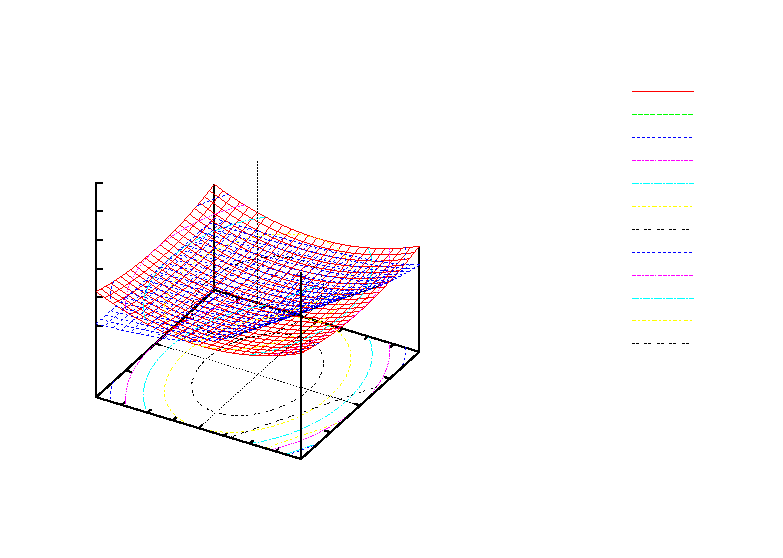
\includegraphics{appc2}}%
    \gplfronttext
  \end{picture}%
\endgroup

 \end{center}\vspace{-15mm}
\end{figure}

The numbers listed below the functions in the key in the upper right corner of the graph are the ``levels'' of the
level curves of the corresponding surface. That is, they are the numbers $c$ such that $f(x,y)=c$.
Because of the large number of level curves, the key was put outside the graph with the
\textbf{set key outside} command.
If you do not want the function key displayed, it can be turned off with this command: \textbf{unset key}\vspace{2mm}

\par\noindent\textbf{PARAMETRIC FUNCTIONS}\vspace{2mm}\\
Gnuplot has the ability to graph surfaces given in various parametric forms. For example, for a surface
parametrized in cylindrical coordinates
\begin{displaymath}
 x=r\cos \theta ~,\quad y=r\sin \theta ~,\quad z=z
\end{displaymath}
you would do the following:\vspace{2mm}

\begin{tabular}{l @{}}
\texttt{set mapping cylindrical}\\
\texttt{set parametric}\\
\texttt{splot \symbol{91}a:b\symbol{93}\symbol{91}c:d\symbol{93} v*cos(u),v*sin(u),f(u,v)}
\end{tabular}\vspace{2mm}

\par\noindent where the variable $u$ represents $\theta$, with $a\le u \le b$, the variable $v$ represents $r$, with
$c\le v\le d$, and $z=f(u,v)$ is some function of $u$ and $v$.

\vspace{3mm}
\hrule width \textwidth height 0.5pt\vspace{2mm}
\par\noindent \emph{\textbf{Example C.2.}} The graph of the helicoid
$z=\theta$ in Example \ref{exmp:helicoid} from Section 1.7 (p. \pageref{exmp:helicoid}) was created using
the following commands:\vspace{2mm}

\begin{tabular}{l @{}}
\texttt{set mapping cylindrical}\\
\texttt{set parametric}\\
\texttt{set view 60,120,1,1}\\
\texttt{set xyplane 0}\\
\texttt{set xlabel "x"}\\
\texttt{set ylabel "y"}\\
\texttt{set zlabel "z"}\\
\texttt{unset key}\\
\texttt{set isosamples 15}\\
\texttt{splot \symbol{91}0:4*pi\symbol{93}\symbol{91}0:2\symbol{93} v*cos(u),v*sin(u),u}
\end{tabular}\vspace{2mm}

\par\noindent The command \textbf{set xyplane 0} moves the $z$-axis so that $z=0$ aligns with the $xy$-plane (which
is \emph{not} the default in Gnuplot). Looking at the graph, you will see that $r$ varies from $0$ to $2$, and $\theta$
varies from $0$ to $4\pi$.\vspace{2mm}
\hrule width \textwidth height 0.5pt\vspace{1mm}
\vspace{3mm}

\par\noindent\textbf{PRINTING AND SAVING}\vspace{2mm}\\
In Windows, to print a graph from Gnuplot right-click on the titlebar of the graph's window, select ``Options'' and then
the ``Print..'' option. If that does not work on your version of Gnuplot, then go to the File menu on the main Gnuplot menubar,
select ``Output Device ...'', and enter \path{pdf} in the \emph{Terminal type?} textfield, hit OK. That will
allow you to print the graph as a PDF file.

To save a graph, say, as a PNG file, go to the File menu on the main Gnuplot menubar,
select ``Output Device ...'', and enter \path{png} in the \emph{Terminal type?} textfield, hit OK. Then, in the
File menu again, select the ``Output ...'' option and enter a filename (say, graph.png) in the \emph{Output
filename?} textfield, hit OK. Now run your splot command again and you should see a file called
graph.png in the current directory (usually the directory where \path{wgnuplot.exe} is located, though you can change
that setting using the ``Change Directory ...'' option in the File menu).\\

\par\noindent In Linux, to save the graph as a file called graph.png, you would issue the following
commands:\vspace{2mm}

\begin{tabular}{l @{}}
\texttt{set terminal png}\\
\texttt{set output 'graph.png'}
\end{tabular}\vspace{2mm}

\par\noindent and then run your splot command. There are many terminal types (which determine the output format). Run
the command \textbf{set terminal} to see all the possible types. In Linux, the \textbf{postscript} terminal type is
popular, since the print quality is high and there are many PostScript viewers available.
\vspace{2mm}

\par\noindent To quit Gnuplot, type \textbf{quit} at the \textbf{\path{gnuplot>}} command prompt.
